\documentclass{beamer}

\usepackage{préambule}
\usetikzlibrary{calc}

\newcommand\scalemath[2]{\scalebox{#1}{\mbox{\ensuremath{\displaystyle #2}}}}
\renewcommand{\widevec}[1]{\scalemath{0.85}{\overrightarrow{#1}}}

\setbeamersize{
	text margin left=0.3cm,
	text margin right=0.3cm
}
\setlength{\leftmargini}{0.5cm}
\setlength{\leftmarginii}{0.3cm}

\begin{document}

\begin{frame}
	\footnotesize
	\begin{multicols}{2}
		\uline{Sujet A}
		\vspace*{-0.5cm}
		\begin{center}
			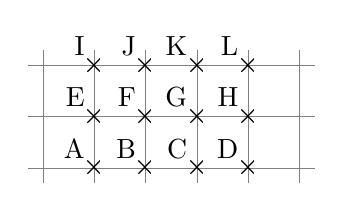
\begin{tikzpicture}[scale=0.65]
				\coordinate (A) at (0,0);
				\coordinate (B) at (1,0);
				\coordinate (C) at (2,0);
				\coordinate (D) at (3,0);
				\coordinate (E) at (0,1);
				\coordinate (F) at (1,1);
				\coordinate (G) at (2,1);
				\coordinate (H) at (3,1);
				\coordinate (I) at (0,2);
				\coordinate (J) at (1,2);
				\coordinate (K) at (2,2);
				\coordinate (L) at (3,2);
				\draw[very thin,gray] (-1.3,-0.3) grid (4.3,2.3);

				\foreach \p in {A,B,C,D,E,F,G,H,I,J,K,L} {
						\node at (\p) {×};
						\node[above left] at (\p) {\p};
					}
			\end{tikzpicture}
		\end{center}
		\begin{enumerate}
			\item \begin{enumerate}[a.]
				      \item Donner deux vecteurs égaux à $\widevec{LD}$.
				      \item Donner un représentant de $\widevec{AB} + \widevec{BG}$.
				      \item Donner deux représentants de $\widevec{EG} + \widevec{HC}$.
				      \item Donner deux représentants de $\widevec{KD} + \widevec{FK} + \widevec{CG}$.
			      \end{enumerate}
			\item Construire un triangle ABC rectangle en A, avec AB = 6cm et AC = 5cm.
			      \begin{enumerate}[a.]
				      \item Construire le point D tel que $\widevec{AD} = \widevec{CB}$.
				      \item Construire le point E tel que $\widevec{BE} = \widevec{AC} + \widevec{AB}$.
			      \end{enumerate}
		\end{enumerate}

		\setlength{\columnseprule}{0.7pt}
		\columnbreak
		\setlength{\columnseprule}{0pt}

		\uline{Sujet B}
		\vspace*{-0.5cm}
		\begin{center}
			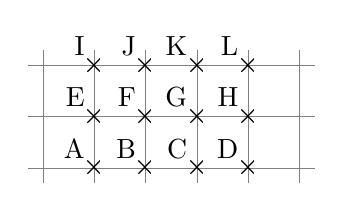
\begin{tikzpicture}[scale=0.65]
				\coordinate (A) at (0,0);
				\coordinate (B) at (1,0);
				\coordinate (C) at (2,0);
				\coordinate (D) at (3,0);
				\coordinate (E) at (0,1);
				\coordinate (F) at (1,1);
				\coordinate (G) at (2,1);
				\coordinate (H) at (3,1);
				\coordinate (I) at (0,2);
				\coordinate (J) at (1,2);
				\coordinate (K) at (2,2);
				\coordinate (L) at (3,2);
				\draw[very thin,gray] (-1.3,-0.3) grid (4.3,2.3);

				\foreach \p in {A,B,C,D,E,F,G,H,I,J,K,L} {
						\node at (\p) {×};
						\node[above left] at (\p) {\p};
					}
			\end{tikzpicture}
		\end{center}
		\begin{enumerate}
			\item \begin{enumerate}[a.]
				      \item Donner deux vecteurs égaux à $\widevec{BJ}$.
				      \item Donner un représentant de $\widevec{EF} + \widevec{FG}$.
				      \item Donner deux représentants de $\widevec{KF} + \widevec{HG}$.
				      \item Donner deux représentants de $\widevec{CA} + \widevec{EB} + \widevec{FG}$.
			      \end{enumerate}
			\item Construire un triangle ABC rectangle en A, avec AB = 5cm et AC = 6cm.
			      \begin{enumerate}[a.]
				      \item Construire le point D tel que $\widevec{AD} = \widevec{CB}$.
				      \item Construire le point E tel que $\widevec{BE} = \widevec{AC} + \widevec{AB}$.
			      \end{enumerate}
		\end{enumerate}
	\end{multicols}
\end{frame}

\begin{frame}
	\footnotesize\color{red}
	\uline{Sujet A : CORRECTION}

	\begin{enumerate}
		\item \begin{enumerate}[a.]
			      \item $\widevec{KC}$ et $\widevec{JB}$
			      \item $\widevec{AG}$
			      \item $\widevec{EB}$ et $\widevec{FC}$
			      \item $\widevec{IK}$ et $\widevec{EG}$
		      \end{enumerate}
		\item \

		      \begin{center}
			      \begin{tikzpicture}[scale=0.5]
				      \coordinate (A) at (0,0);
				      \coordinate (B) at (6,0);
				      \coordinate (C) at (0,5);
				      \coordinate (D) at ($(A) + (B) - (C)$);
				      \coordinate (E) at ($(B) + (C) - (A) + (B) - (A)$);

				      \draw (A) -- (B) -- (C) -- (A);
				      \draw[red,->] (A) -- (D);
				      \draw[red,->] (B) -- (E);

				      \foreach \p/\dir in {A/below,B/below,C/left,D/below,E/left} {
						      \node[\dir] at (\p) {\p};
					      }
			      \end{tikzpicture}
		      \end{center}
	\end{enumerate}
\end{frame}

\begin{frame}
	\footnotesize\color{red}
	\uline{Sujet B : CORRECTION}

	\begin{enumerate}
		\item \begin{enumerate}[a.]
			      \item $\widevec{AI}$ et $\widevec{CK}$
			      \item $\widevec{EG}$
			      \item $\widevec{KE}$ et $\widevec{LF}$
			      \item $\widevec{GC}$ et $\widevec{EA}$
		      \end{enumerate}
		\item \

		      \begin{center}
			      \begin{tikzpicture}[scale=0.5]
				      \coordinate (A) at (0,0);
				      \coordinate (B) at (5,0);
				      \coordinate (C) at (0,6);
				      \coordinate (D) at ($(A) + (B) - (C)$);
				      \coordinate (E) at ($(B) + (C) - (A) + (B) - (A)$);

				      \draw (A) -- (B) -- (C) -- (A);
				      \draw[red,->] (A) -- (D);
				      \draw[red,->] (B) -- (E);

				      \foreach \p/\dir in {A/below,B/below,C/left,D/below,E/left} {
						      \node[\dir] at (\p) {\p};
					      }
			      \end{tikzpicture}
		      \end{center}
	\end{enumerate}
\end{frame}

\end{document}